\documentclass[a4paper, 12pt]{article}
\renewcommand{\baselinestretch}{1.5}
\usepackage{algorithm}
\usepackage{arevmath}     % For math symbols
\usepackage{algpseudocode}
\usepackage{mathtools}
\usepackage{fontspec}
\usepackage{graphicx}
\usepackage{tabularx}
\usepackage{setspace}
\usepackage{longtable}
\usepackage{amsmath}
\usepackage{unicode-math}
\usepackage{capt-of}
\usepackage{sectsty}
\usepackage{stackengine}
\usepackage{hyperref}
\usepackage{caption}
\usepackage{titlesec}
\usepackage{subcaption}
\usepackage{array,ragged2e}
\usepackage[justification=centering]{caption}
\usepackage[format=hang,font={small,bf},labelfont=bf]{caption}
\usepackage{nomencl}
\usepackage{siunitx}
\usepackage{etoolbox}
\makenomenclature
\usepackage[sorting=none]{biblatex} %Imports biblatex package
\addbibresource{ref.bib} %Import the bibliography file
\defbibheading{References}[\bibname]{%
  \section*{\centering #1}%
  \markboth{#1}{#1}}
\newcommand\xrowht[2][0]{\addstackgap[.5\dimexpr#2\relax]{\vphantom{#1}}}
\usepackage[margin=1in]{geometry}
\usepackage{tocloft}

%  \pagestyle{empty}
\setmainfont{Times New Roman}
\captionsetup[figure]{font={small, bf},labelfont={bf},name={Fig.},labelsep=period}
\renewcommand{\algorithmicrequire}{\textbf{Input:}}
\renewcommand{\algorithmicensure}{\textbf{Output:}}
\renewcommand{\nomname}{\makebox[\linewidth]{Nomenclature}}%
\renewcommand{\contentsname}{\hfill\bfseries\Large Contents\hfill}
\renewcommand{\cftaftertoctitle}{\hfill}
\sectionfont{\fontsize{18}{18}\selectfont}
\setcounter{tocdepth}{4}
\setcounter{secnumdepth}{4}
\titleformat{\paragraph}
{\normalfont\normalsize\bfseries}{\theparagraph}{1em}{}
\titlespacing*{\paragraph}
{0pt}{3.25ex plus 1ex minus .2ex}{1.5ex plus .2ex}

\begin{document}
\pagenumbering{roman}
\setcounter{page}{1}
\tableofcontents
\newpage
\begin{center}
\phantomsection
\listoftables
\addcontentsline{toc}{section}{\listtablename}
\end{center}
\newpage
\begin{center}
\phantomsection
\listoffigures
\addcontentsline{toc}{section}{\listfigurename}
\end{center}
%% This code creates the groups
% -----------------------------------------

\renewcommand\nomgroup[1]{%
  \item[\bfseries
  \ifstrequal{#1}{E}{Non-English Alphabets}{%
  \ifstrequal{#1}{H}{English Alphabets}{%
  \ifstrequal{#1}{I}{Abbreviations}{%
  \ifstrequal{#1}{O}{Other symbols}{}}}}%
]}
% -----------------------------------------
%% This will add the units
%----------------------------------------------
\newcommand{\nomunit}[1]{%
\renewcommand{\nomentryend}{\hspace*{\fill}#1}}
%----------------------------------------------
\newpage
\phantomsection{}
\printnomenclature
\nomenclature[E]{\(\alpha\)}{Alpha}
\nomenclature[E]{\(\beta\)}{Beta}
\nomenclature[E]{\(\epsilon\)}{Epsilon}
\nomenclature[E]{\(\sigma\)}{Sigma}
\nomenclature[E]{\(\sum\)}{Uppercase Sigma}
\nomenclature[E]{\(\omega\)}{Omega}

\nomenclature[H]{\(e\)}{Euler's constant \nomunit{\(2.71828\)}}



\nomenclature[I]{\(ANN\)}{Artificial Neural Network}
\nomenclature[I]{\(ARCH\)}{Autoregressive Conditional Heteroscedasticity}
\nomenclature[I]{\(AUC\)}{Area Under Curve}

\nomenclature[I]{\(BN\)}{Bayesian Network}
\nomenclature[I]{\(CART\)}{Classification and Regression Trees}
\nomenclature[I]{\(DAG\)}{Directed Acyclic Graph}
\nomenclature[I]{\(DT\)}{Decision Tree}
\nomenclature[I]{\(EDA\)}{Exploratory Data Analysis}
\nomenclature[I]{\(GARCH\)}{Generalized Autoregressive Conditional Heteroskedasticity}
\nomenclature[I]{\(KNN\)}{K-Nearest Neighbours}
\nomenclature[I]{\(LCR\)}{Liquidity Coverage Ratio}
\nomenclature[I]{\(LR\)}{Logistic Regression}
\nomenclature[I]{\(LDA\)}{Linear Discriminant Analysis}
\nomenclature[I]{\(MLP\)}{Multilayer Perceptron}
\nomenclature[I]{\(MSE\)}{Mean Squared Error}
\nomenclature[I]{\(NSFR\)}{Net Stable Funding Ratio}
\nomenclature[I]{\(NPA\)}{Non Performing Assets}
\nomenclature[I]{\(RBI\)}{The Reserve Bank of India}
\nomenclature[I]{\(RF\)}{Random Forest}
\nomenclature[I]{\(ROC\)}{Receiver Operating Characteristics}
\nomenclature[I]{\(SVM\)}{Support Vector Machine}
\nomenclature[I]{\(VAR\)}{Value at Risk}
\addcontentsline{toc}{section}{Nomenclature}
\newpage
\begin{center}
\phantomsection
\section*{\centering Abstract}
\addcontentsline{toc}{section}{Abstract}
\end{center}
\textit{
{\fontsize{10pt}{10pt}\selectfont In today's era, the data volume is exploding and each second, new data is created and stored on a server or the cloud. This increases the risk of data breaching. Data breaching is an issue that exists at an enterprise level as well as on a day-to-day basis. Protection of data is of significant importance and biometric verification is a commonly used approach to implement data security. Biometric systems are categorized majorly into two types - unimodal and multimodal systems. Unimodal approaches make use of a single biometric trait including face, fingerprint, gait, voice, etc. However, there exists a high number of limitations to this system thus the multimodal system is adapted. The multimodal system performs the fusion of two or more biometric traits and makes the decision based on it. The fusion approach has various algorithms associated with it. These methods and limitations are analyzed in detail and are followed by references to studies showing their results in the field of biometric systems. <TODO: Replace Abstract>
}
}
\vskip 0.1in
\noindent\
\emph{
{\fontsize{10pt}{10pt}\selectfont \textbf{Keywords:}  Banking - Risk Management - Machine Learning - Credit Score}}

\begin{center}
\newpage
\pagenumbering{arabic}
\setcounter{page}{1}
\section{\centering Introduction}
\end{center}
\vskip 0.25in
The banking industry is an essential part of the global economy handling over 150 trillion U.S Dollars worth of global assets. Amidst the economic recession caused due to the COVID-19 pandemic, the total value of banking-related fraud in India doubled from Rs 71,534 Crores in 2018-19 to Rs 1,38,422 Crores in the fiscal year  2020-21 [1]. Global recessions like the 2008 Financial Crisis and the recent COVID-19 pandemic slows down economic output and put a lot of pressure on financial institutions, especially banks. Having a strong infrastructure to manage and mitigate financial risk becomes crucial to keeping the global economic engine running.
\vskip 0.2in
\noindent
Over the last few decades, advancements in Machine Learning have been extensively utilized to help in risk management tasks. With almost all financial instruments running in a digital form, machine learning models are employed extensively to detect fraud, predict commodity prices, track inflation etc. A lot of research has been done academically and in the industry since the 2008 Financial Crisis to build state of the art models for various risk management activities. This report presents a summary of multiple machine learning techniques that are used to solve a variety of risk management related problems.
\vskip 0.2in
\subsection{Applications}
Risk management is a 17.1 Billion U.S. Dollar industry responsible for handling inflation, financial frauds, cyber threats, market volatility etc. [2]. Machine Learning models significantly improve the accuracy of existing risk management tasks and can do so globally by working on petabytes of data that the banking sector produces daily. Typical applications of machine learning in risk management tasks include:

\begin{itemize}
  \item \textbf{Credit Risk:} Determining if the borrower can repay the loan.
  \item \textbf{Market Risk:} Predicting volatility and movement in commodity and equity markets.
  \item \textbf{Financial Fraud Risk:} Identifying money laundering patterns from transactions.
  \item \textbf{Liquidity Risk:} Identifying stability of sectors before investing in financial instruments
  \item \textbf{Operational Risk:} Detecting Fraud and suspicious transactions
\end{itemize}






\vskip 0.2in
\subsection{Motivation}
Risk Management is essential for a country's economy. The Reserve Bank of India (RBI) reported the presence of about Rs. 900 Thousand Crores of Non-Performing Assets (NPA) in 2020 in the Indian banking sector [3]. These are essentially bank loans that are in default or arrears. This amount of loss is roughly equivalent to the cost to build an international airport in India. Machine Learning plays a monumental role in reducing exposure to such risks, which can significantly impact national and global economies.
\vskip 0.2in
\subsection{Objectives}
This report aims to summarize the work done in risk management in the banking sector from a machine learning point of view. Additionally, this report also presents a case study comparing the performance of different machine learning models to evaluate credit risk on a single dataset.
\vskip 0.2in
\subsection{Organization of Report}
<TODO: Write This>
This report is subdivided into four chapters. The first chapter gives the introduction to biometric authentication, its applications, motivations, and the objective of this report. The second chapter gives a basic understanding of the tasks within the biometric system, a brief explanation of the unimodal and multimodal biometric system followed by terminologies used in biometric authentication. The third chapter contains an in-depth understanding of the various implementations of popular unimodal and multimodal biometric techniques that elevate data security. The final chapter covers the conclusion for the report outlining the machine learning and statistical approaches used for biometric authentication.
\newpage

\section{\centering{Theoretical Background}}
\vskip 0.25in
This chapter is subdivided into two parts. The first part is a brief outline of standard machine learning models and terminologies. The second part explains various terminologies related to finance, banking and risk management.
\vskip 0.2in
\subsection{Machine Learning Algorithms}
\subsubsection{Logistic Regression (LR)}
\begin{center}
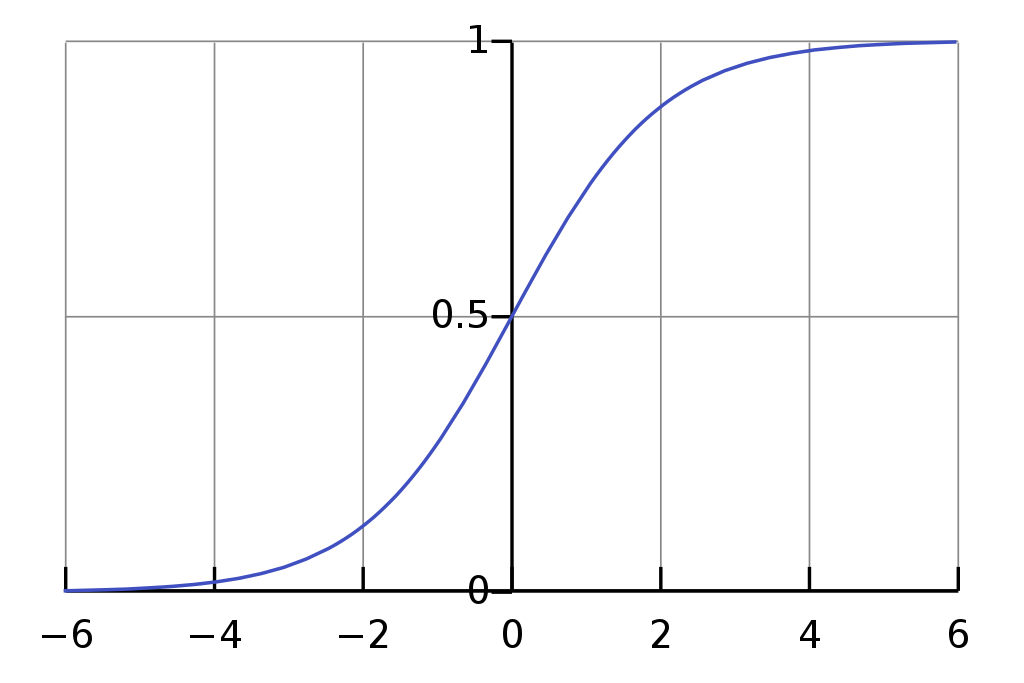
\includegraphics[scale=0.3]{lr.png}
\captionof{figure}{Logistic function curve}
\label{fig:lr}
\end{center}
In statistics, LR models the probability of a specific class or event happening. This probability estimate is further used for binary classification and with minor extensions to perform multi-class classification. The algorithm is based on a logistic function which is a sigmoidal curve. It takes a real-valued input and outputs a number between zero and unity (Fig. \ref{fig:lr}). This output is interpreted as the probability of the task. Mathematically, the logistic function is represented as follows:
\begin{equation}
\sigma(t) = \frac{e^t}{1 + e^t} = \frac{1}{1 + e^{-t}}
\end{equation}
If \(t\) is derived from a single independent linearly varying variable \(x\), the generalized logistic function can be represented as follows:
\begin{equation}
    t = \beta_0 + \beta_1x
    \end{equation}
    \begin{equation}
    p(x) = \sigma(t) = \frac{1}{1 + e^{\beta_0 + \beta_1x}}
\end{equation}
\vskip 0.2in
\subsubsection{Decision Tree (DT)}
\noindent Decision Tree Learning involves the construction of DTs, which will be traversed to conclude a given set of observations of data points. Classification Trees are models where the predicted outcome is discrete. Decision Tree training algorithms work in a top-down fashion to split the data set at every stage using a specific metric. Popular decision trees and their splitting metrics are discussed below.
\vskip 0.2in
\noindent\textbf{Classification and Regression Tree (CART)} \\
\noindent CART model uses the Gini Impurity Index \(I_G\) as its splitting parameter, which is computed for \(j\) classes as follows:
\begin{equation}
    I_{G}(p) = 1 - \sum_{i = 1}^{j} p_i^2
\end{equation}
\vskip 0.2in
\noindent\textbf{Information Gain based DTs} \\
\noindent DT models like ID3, C4.5 and C5.0 use information gain, which is based on the entropy  of the dataset. Mathematically Entropy \(H\) and Information Gain \(IG\) for \(j\) classes are defined as below:

\begin{equation}
    H(T) = - \sum_{i=1}^{j} p_i \log_2 p_i
\end{equation}

\begin{equation}
    IG(T, a) =  H(T) - H(T|a)
\end{equation}

\vskip 0.2in
\subsubsection{Random Forests (RF)}
\noindent RFs are constructed using ensemble learning on DTs. The majority output of the decision trees is considered the output of an RF in a classification task. The mean of all outputs is taken for a regression task. RFs are used as a corrective measure for overfitting of DT based models.

\vskip 0.2in
\subsubsection{Support Vector Machine (SVM)}
\begin{center}
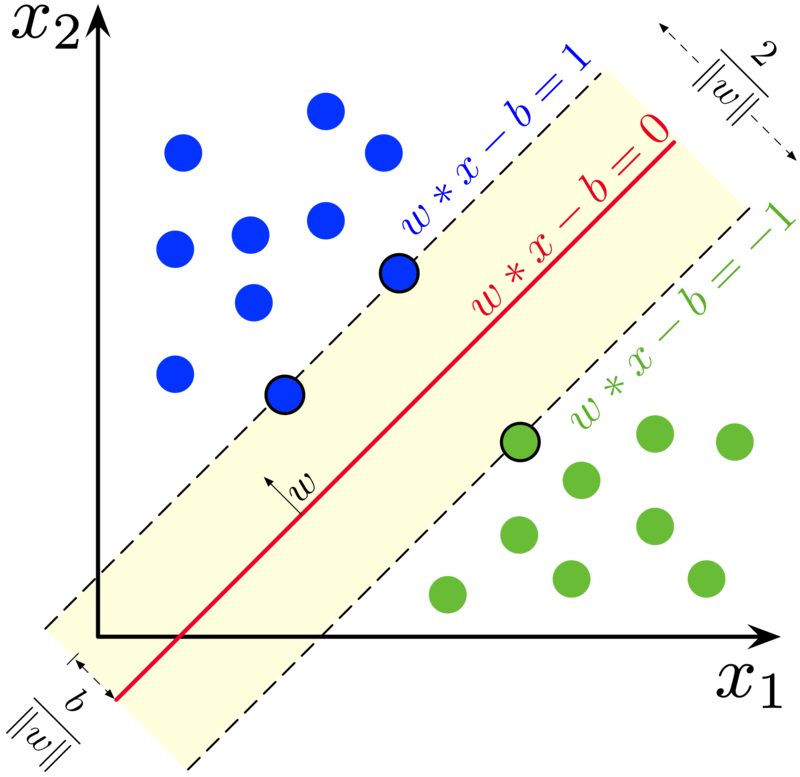
\includegraphics[scale=1.8]{svm-1.png}
\captionof{figure}{Hyperplane construction in SVM}
\label{fig:svm-1}
\end{center}

\noindent SVMs are supervised learning models used for regression and classification tasks. For classification, two hyperplanes are constructed, separating linearly separable data classes. The hyperplane at the midway of these two planes is the maximum hyperplane which acts as a classification boundary (Fig. \ref{fig:svm-1}).

\vskip 0.2in
\begin{center}
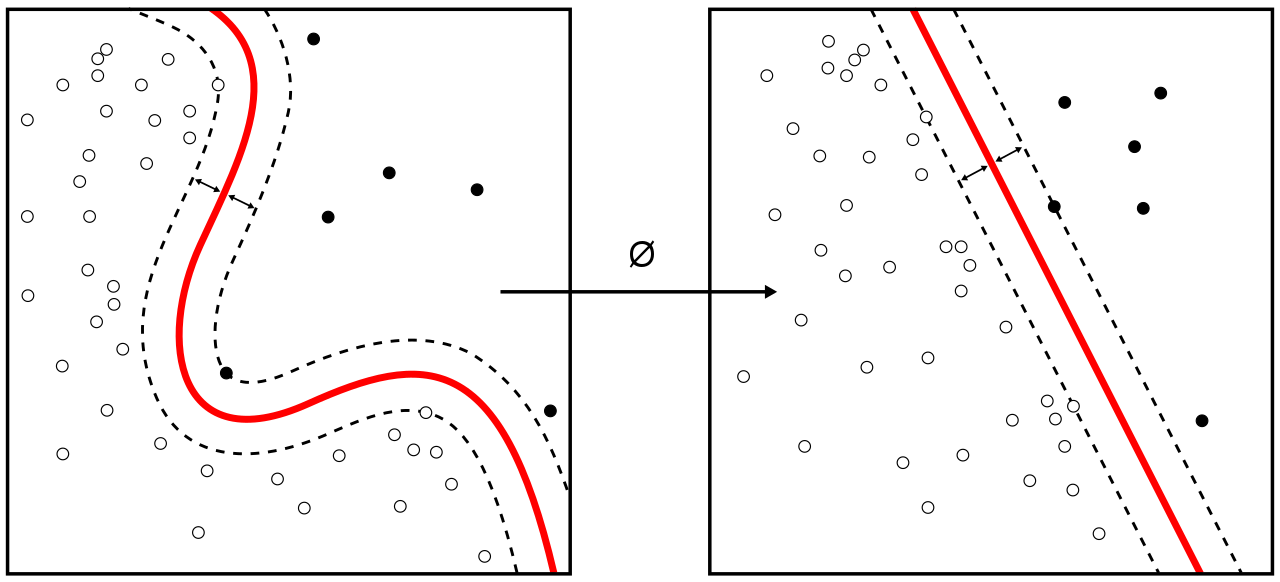
\includegraphics[scale=0.2]{svm-2.png}
\captionof{figure}{Kernel mapping to linear boundaries}
\label{fig:svm-2}
\end{center}
\noindent 
For non-linear data, a kernel is used, which is a function mapping the data into higher dimensional linear feature space (Fig. \ref{fig:svm-2})


\vskip 0.2in
\subsubsection{K-Nearest Neighbours (KNN)}
\begin{center}
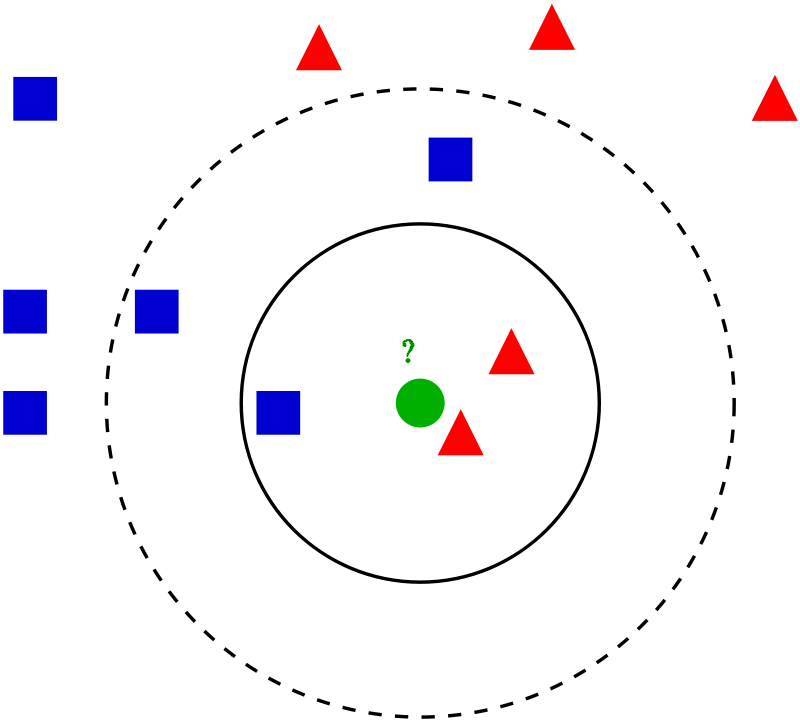
\includegraphics[scale=0.3]{knn.png}
\captionof{figure}{Example of KNN}
\label{fig:knn}
\end{center}
\noindent KNN is a supervised algorithm for supervised classification and regression tasks. KNN works by finding the \(K\) closest data points to a given query point. The output is the most frequent label for classification and the mean of the label for regression tasks. The value of \(K\) is user-defined as a hyperparameter, and the distance metric is euclidean or hamming distance depending on the context of the dataset.

\vskip 0.2in
\subsubsection{Bayesian Network (BN)}
\noindent A BN is a Directed Acyclic Graph (DAG) used to represent the probabilistic dependencies of a collection of random variables. Each node of the BN represents a random variable, and each edge between the nodes represents the conditional probability between the nodes, which is derived from the Bayes theorem:
\begin{equation}
    P(A|B) = \frac{P(B|A)P(A)}{P(B)}
\end{equation}
As an example, consider the BN in (Fig. \ref{fig:bn}), modelling the conditions when the grass can be wet. If it rains or the sprinklers are active, there is a higher probability of grass being wet. Moreover, if it is raining, the probability of the sprinkler being kept active is lesser.
\begin{center}
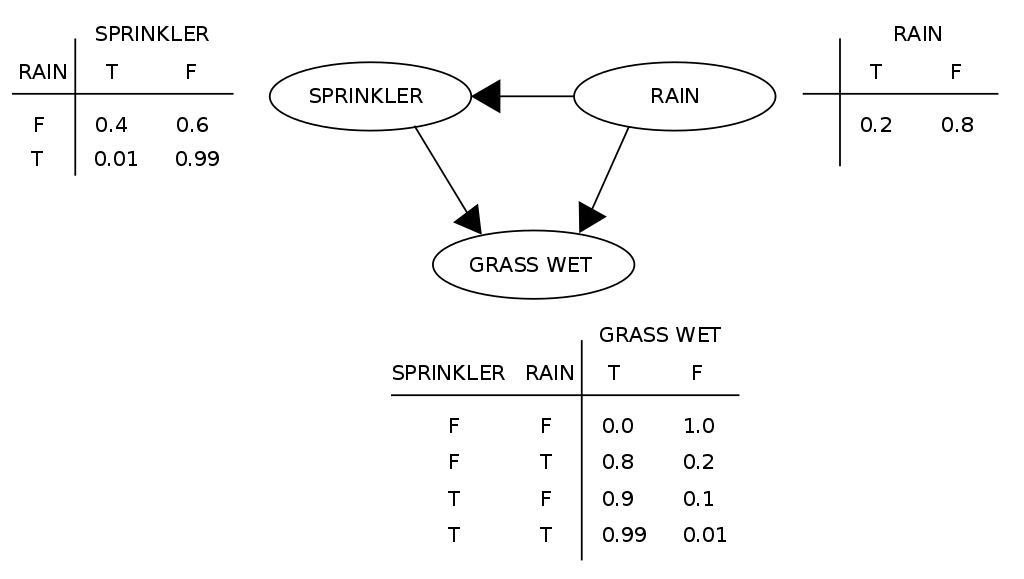
\includegraphics[scale=0.3]{bn.png}
\captionof{figure}{Example of BN}
\label{fig:bn}
\end{center}

\vskip 0.2in
\subsubsection{Linear Discriminant Analysis (LDA)}
\begin{center}
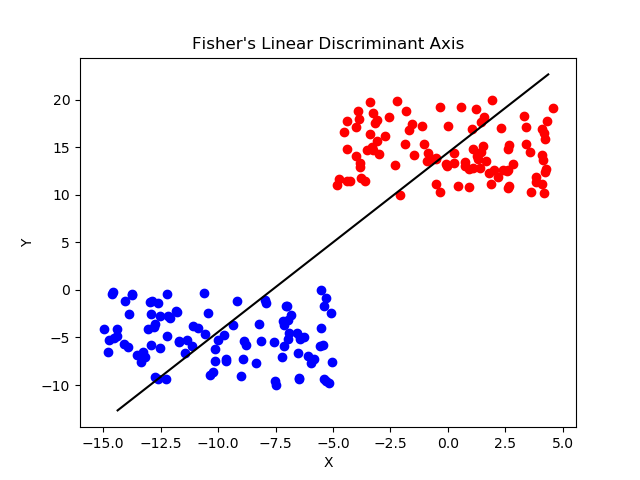
\includegraphics[scale=0.8]{lda.png}
\captionof{figure}{Fisher's LDA Visualization}
\label{fig:lda}
\end{center}

\noindent LDA is used for dimensionality reduction, especially for supervised classification tasks to separate two or more classes spatially. LDA takes a component of the data points on a single axis tuned to maximize the distance between two classes and minimize the variation within members of a single class.

\vskip 0.2in
\subsubsection{Artificial Neural Networks (ANN)}

\noindent ANNs are machine learning models mimicking biological neural networks. An ANN consists of neuron layers where each layer contains an array of artificial neurons. These neurons are essentially mathematical functions that take input values from previous layers and are tunable using a set of weights and biases. ANNs are used for supervised, unsupervised as well as reinforcement learning tasks.

\begin{center}
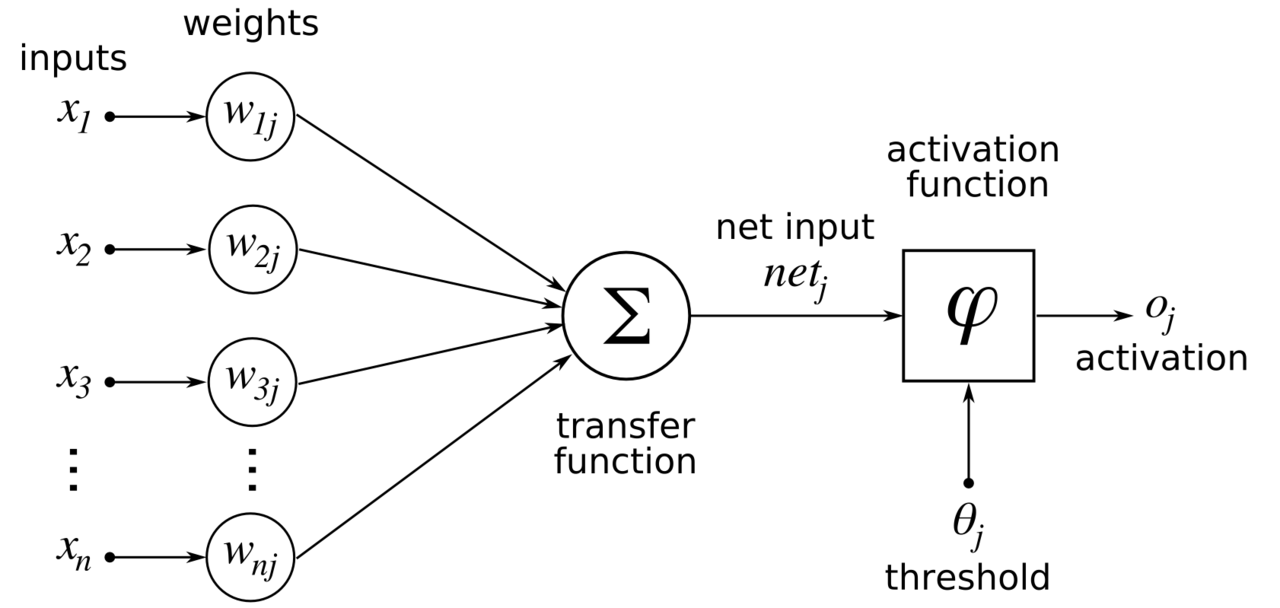
\includegraphics[scale=0.38]{ann.png}
\captionof{figure}{Single neuron in an ANN}
\label{fig:ann}
\end{center}

\vskip 0.2in
\noindent\textbf{Multilayer Perceptron (MLP)} \\
\noindent MLPs are a class of feedforward ANNs where the connections between layers of neurons are unidirectional and acyclic. Each neuron is an activation function like hyperbolic tan, logistic function and rectifier function.
\begin{equation}
    y(v_i) = \tanh(v_i)
\end{equation}
\begin{equation}
    y(v_i) = \frac{1}{1 + e^{v_i}}
\end{equation}
\begin{equation}
    y(v_i) = \max(0, v_i)
\end{equation}

\vskip 0.2in
\subsection{Overview Banking and Risk Management Terminologies}
\subsubsection{Risk}
\noindent Risk in finance is defined as uncertainty or volatility of unexpected outcomes, representing the value of assets, equity, or earnings. This includes both positive as well as negative outcomes. A higher return is associated with a more significant variability of outcomes [6]. Risk is broadly classified into Credit Risk, Market Risk, Liquidity Risk and Operational Risk.

\vskip 0.2in
\subsubsection{Market Risk}
\noindent Market risk is the risk of the movement of market prices. Prices of market parameters that fluctuate randomly include equity indexes, commodity prices, interest rates and foreign exchange rates [4].

\vskip 0.2in
\noindent\textbf{Time Series Forecasting} \\
\noindent Time Series Forecasting is used to predict the market price movement. It involves conceptualizing statistical and machine learning models to predict future values based on previously observed values.

\vskip 0.2in
\noindent\textbf{Innovation} \\
\noindent Innovation is the difference between a forecast made by a statistical algorithm and the actual value for a time-varying function.

\vskip 0.2in
\noindent\textbf{Heteroscedasticity} \\
\noindent Heteroscedasticity is the variance or volatility observed in a time-varying random function.

\vskip 0.2in
\subsubsection{Liquidity Risk}
\noindent Liquidity is the ease with which a financial instrument can be exchanged for money without losing value. High liquidity indicates a high supply and demand for an asset, which means there will always be buyers and sellers. Liquidity risk is the uncertainty linked with the outcome and possible losses of such an asset transaction into funds [7].

\vskip 0.2in
\noindent\textbf{Measuring Liquidity} \\
\noindent Liquidity is measured using ratios like Liquidity Coverage Ratio (LCR) and Net Stable Funding Ratio (NSFR). LCR measures the number of liquid assets a bank has to cover for any short term liquid fund requirements. NSFR, on the other hand, measure a bank's long term resilience to liquidity risks. Basel Norms require that both the ratios must be maintained above 100\% by banks.

\begin{equation}
    LCR = \frac{\text{stock of high quality liquid assets}}{\text{total net cash} - \text{flow over the next 30 days}}
\end{equation}

\begin{equation}
    NSFR = \frac{\text{available amount of stable funding}}{\text{required amount of stable funding}}
\end{equation}

\vskip 0.2in
\subsubsection{Operational Risk}
\noindent Operational Risk is the risk associated with failures in internal procedures, external events, and infrastructure. Fraud detection, cyber security attacks, suspicious transaction detection, money laundering all come under the radar of operational risk [4].

\vskip 0.2in
\noindent\textbf{Money Laundering} \\
\noindent Money Laundering converts substantial amounts of funds earned from crimes and terrorism into origination from a legitimate source. This is accomplished by routing transactions through numerous layers of legal transactions to hide the natural source of income.

\vskip 0.2in
\subsection{Summary}
In conclusion, this chapter briefly introduces various concepts and terminologies that would be a prerequisite for Chapter 3 and Chapter 4. Machine learning algorithms are used to solve a vast array of economics, banking, and risk management problems.

\newpage
\section{\centering Literature Review}
\vskip 0.25in
This chapter discusses various contributions of researchers and scholars for Risk Management in Banking using Machine Learning Models.

\vskip 0.2in
\subsection{Credit Risk}
Credit Risk analysis is the fundamental problem of the lending economy, with initial efforts dating back to the 20th century. The financial recessions of the 21st century and the ever-increasing complexity of regulatory constraints have led to increased academic and business efforts towards the problem. From a Machine Learning perspective, evaluating credit risk involves binary classification: Determining if a potential customer is credit-worthy from their financial history.

\vskip 0.2in
\subsubsection{Traditional Machine Learning Algorithms for Credit Scoring}
\noindent A family of statistical frameworks have been adopted since the early 1900s for credit scoring potential borrowers. Among the traditional classifiers, SVMs have yielded significantly better results.
\\
\\
\noindent Bellotti et al. tested the performance of SVMs for credit score classification and contrasted the results with traditional approaches [8]. The paper compares the performance of different algorithms like LR, SVM, LDA and KNN. The work concluded with LDA and SVM reporting the highest AUC scores for the ROC curves when trained on a dataset of about 25,000 over three months of 2004 for credit card based lending [8]. However, SVMs are very sensitive to the outliers of the datasets. Wang et al. introduced a fuzzy SVM algorithm for the classification task to reduce this sensitivity and increase the generalization of the data [13].

\vskip 0.2in
\subsubsection{Neural Networks for Credit Scoring}
\noindent Early works in the area primarily included the use of SVM based algorithms. However, with larger datasets, training becomes computationally expensive [10]. ANNs have been widely researched for credit scoring [11, 12]. Several Ensemble methods have been employed to improve the accuracy of the ANN models [9].
\\
\\
Angelini et al. used ANNs to determine credit risk among small businesses as credit borrowers [14]. The work proposes a real-world dataset of Italian businesses and provides a comprehensive network performance analysis for various neuron configurations.
\\
\\
Tsai et al. employed a single MLP classifier as a benchmark for prediction accuracy and compared the performance with multiple classifiers in the ensembled form [9]. The paper also reports the variation in accuracy by modifying training configuration parameters like the number of epochs, network architecture, and the number of classifiers for ensembling. The analysis is performed on the publicly available Australian, German and Japanese credit datasets.


\vskip 0.2in
\subsection{Market Risk}
\noindent Market risk deals with the volatility of indices. Value at Risk (VAR) estimates the worst loss that will not exceed in a particular time frame. It captures the combined effect of underlying volatility and exposure to financial risks. Volatility estimation is a part of the time series forecasting domain. ANNs excel at these learning problems compared to traditional methods. A commonly used forecasting framework for time series is the Generalized Autoregressive Conditional Heteroskedasticity (GARCH) model [16]. It is derived from the Autoregressive Conditional Heteroscedasticity (ARCH) model, which predicts the volatility of innovation or error term as a function of previous error terms.
\\
\\
The volatility at time \(t\) is given as a function of prior error terms as:

\begin{equation}
    \sigma_t^2 = \alpha_0 + \sum_{i = 1}^{n} \alpha_i \epsilon_{t - i}^2
\end{equation}

\noindent GARCH model also considers the volatility of prior time to predict the current volatility:

\begin{equation}
    \sigma_t^2 = \ \omega + \sum_{i = 1}^{n} \alpha_i \epsilon_{t - i}^2 + \sum_{i = 1}^{p} \beta_i \sigma_{t - i}^2
\end{equation}

\noindent Zhang et al. proposed a model to calculate the VAR (volatility) in an index from the GARCH model using ANNs [15]. The paper also presents a comparative analysis with other models like just GARCH and SVM to predict volatility.

\vskip 0.2in
\subsection{Liquidity Risk}
\noindent Liquidity risk is the risk of not being equipped to raise capital when required. Trading of financial instruments and assets enable the raising of capital to banking institutions. Such funding is known as funding liquidity. When it is difficult to borrow or raise money, liquidity risk comes into play. For example, banks faced heavy losses in the 2008 crisis when assets were trading at heavily discounted rates due to the crash and the banks urgently needed funds to keep their businesses running.
\\
\\
\noindent Machine learning can solve several liquidity risk factors. ANNs can be used to estimate a risk measure. Approximation of general risk trends and discovery of principal risk determinants can be made using ANNs. BN can be used to predict the probability of a liquidity risk event happening.  By using distributive estimation, the ANN and BN implementations could identify the most critical liquidity risk factors.
\\
\\
\noindent Tavana et al. used a combination of ANN and BN to determine liquidity risk (LCR and NSFR) from a real-world dataset of a U.S. bank focusing mainly on loans for eight consecutive years. The ANN was used to approximate the general trend of liquidity risk and find the influential factors. Further, the BN was used to find the most influential factor from the data filtered by the ANN [19].

\vskip 0.2in
\subsection{Operational Risk}
\noindent Operational arises due to malfunctions in internal and external processes. Machine Learning is used in an operational context to detect such malfunctions. Fraud detection is a significant area of focus of operational risk management.
\\
\\
\noindent Money laundering is the malpractice of hiding illegal sources of income by layering lawful transactions on such sources. This is done by routing money through many complicated but legitimate transactions to conceal the actual source. These funds are further used to support criminal, war and terrorist activities.
\\
\\
\noindent Sudjianto et al. employed clustering algorithms to segment customers based on transaction activity [18]. The work combines clustering and profiling to perform unsupervised peer group analysis (PGA) [20]. These segments are used for analyzing if the group of customers were involved in money laundering. Another challenge in identifying fraud is to flag suspicious transactions first and then perform an anti-money laundering investigation. The paper also presents classifiers like LR, SVM, CART, C4.5, C5.0 and RF for determining illegal transactions.
\\
\\
\noindent Villabos et al. has done comparable work on money laundering detection using ANN, SVM and C5.0 based classifiers [20]. The experiments were performed on a Latin American financial institution dataset, and decision tree-based classifiers excelled at the task compared to other models. 


\newpage
\section{\centering Conclusion}
\vskip 0.25in
In today's era, the data volume is exploding and each second, new data is created and stored on a server or the cloud. This increases the risk of data breaching and the need for data security. The report outlines the method and approaches by which biometric authentication helps with the verification of identity. This further helps in preventing data breaching by allowing authorized personnel for specific data usage. Furthermore, the report outlines the advancements in biometric authentication from unimodal systems to multimodal systems. The evaluation characteristics of the biometrics system include universality, performance, etc, and evaluation metrics such as EER, FAR, and FRR is outlined in the report. Based on these evaluations, the performance of the system was understood and it is observable that the multimodal systems perform better than the unimodal system. 
\vskip 0.2in
\noindent Among the unimodal systems, various approaches and research has been discussed for face, fingerprint, DNA, brain, heart, and voice verification. It is observable that fingerprint is one of the most common approaches and both face and fingerprint have had advancements in their verification approach. It makes use of deep learning models, SVM classifiers and convolutional models, etc. Among the various classifiers and regression models, it is observed that SVM classifiers perform the best for verification purposes except for heart biometric verification where DT supersedes SVM in performance.
\vskip 0.2in
\noindent Among the multimodal systems, the approaches under fusion at the scoring level have been discussed. For each approach, i.e., classification and combination, research has been discussed and outlined in the report. For the combinational approach, the process is neatly outlined on how the matching score is calculated based on the normalization score of each biometric trait. For the classification approach, various classifiers have been tested such as SVM, GMM, and ANN where SVM supersedes the other fusion classifiers in performance in terms of FAR and FRR.  With the current pace of advancement in technology, significant improvements within the field of unimodal and multimodal biometric systems are expected. 

\newpage
% \textbf{
% {\fontsize{18pt}{18pt}\selectfont References} 
% }\\
% \addcontentsline{toc}{chapter}{References}
% \printbibliography
\phantomsection
\addcontentsline{toc}{section}{References}
\printbibliography[heading={References}, title=References]
\newpage
\phantomsection
\section*{\centering Acknowledgment}
\addcontentsline{toc}{section}{Acknowledgment}
\vskip 0.2in
\raggedright I would like to express my deep gratitude and indebtedness to my seminar guide, Dr. Sankita J. Patel, Assistant Professor, Computer Engineering Department, SVNIT Surat for her valuable guidance, useful feedback and co-operation with a kind and encouraging attitude for the successful completion of this report. I would also like to express a deep sense of gratitude to the Computer Engineering Department faculties for direct or indirect support for the completion of this seminar.
\end{document}
